\section{Alcance}

Definir con precisión el alcance es fundamental para asegurar que el desarrollo se ajuste a los objetivos propuestos y se realice dentro de los recursos y tiempos establecidos. Para ello, en esta sección se delimitarán las funcionalidades, exclusiones y limitaciones que se esperan en este proyecto.

\subsection{Funcionalidades Incluidas}

En la plataforma web se ofrecen las siguientes funcionalidades principales:

\begin{itemize}
    \item \underline{Autenticación segura} mediante las credenciales de \textit{Spotify}.
    \item \underline{\textit{Home} o Panel Inicial} donde se muestran la información y estadísticas básicas de la cuenta.
    \item \underline{Gráficos interactivos} para representar los datos del usuario obtenidos en tiempo real.
    \item Interfaz \underline{intuitiva y responsiva}.
    \item \underline{Cierre de sesión seguro}.
\end{itemize}

\subsection{Exclusiones}

Para establecer expectativas claras sobre el alcance del proyecto, se detallan a continuación las funcionalidades que \textbf{no} serán incluidas en la plataforma web:

\begin{itemize}
    \item No se desarrollarán \underline{aplicaciones nativas de otras plataformas} como móvil, PC, Mac o Linux; el acceso será exclusivamente a través de la web.

    \item Aunque se seguirá un diseño intuitivo, no se implementarán funcionalidades específicas de \underline{accesibilidad avanzada}, como compatibilidad con lectores de pantalla o navegación por teclado.

    \item La plataforma se enfoca exclusivamente en la integración con \textit{Spotify}; se excluyen todos los \underline{otros servicios de streaming} como \textit{Apple Music}, \textit{Deezer}, etc.

    \item No se \underline{almacenarán de forma persistente datos personales} del usuario en servidores propios más allá de lo necesario para la sesión actual; todos los datos se obtendrán directamente de la API de \textit{Spotify} y se manejarán en tiempo real.

    \item Se excluye el desarrollo de funcionalidades relacionadas con la \underline{interacción social} (envío de mensajes, compartir estadísticas, rankings entre usuarios, etc.) dentro o a través de la plataforma, ya que superarían el alcance recogido dentro de un TFG.

    \item La interfaz de usuario estará disponible únicamente en español y no se ofrecerá \underline{soporte para otros idiomas}.
\end{itemize}

\subsection{Limitaciones}

Durante el desarrollo del proyecto, se han identificado las siguientes limitaciones que han afectado al alcance y a las funcionalidades de la web:

\begin{itemize}
    \item Las políticas de seguridad de \textit{Spotify} impiden el \underline{almacenamiento persistente de datos} personales, limitando funcionalidades que requieran conservar información del usuario entre sesiones.

    \item El procesamiento de los datos se ve limitado por los \underline{recursos computacionales} que la nube de \textit{Vercel} ofrece, descartando técnicas avanzadas como el aprendizaje automático.

    \item El \underline{tiempo y los recursos disponibles} para el desarrollo del proyecto son finitos, lo que ha obligado a priorizar funcionalidades esenciales y descartar características adicionales.

    \item Al hacer uso de una API de terceros, todas las funcionalidades necesitan una \underline{conexión} \underline{activa a Internet} para poder funcionar de manera correcta.
\end{itemize}

\section{Gestión de Tareas}

Una vez definido el alcance, es necesario detallar las tareas requeridas para el desarrollo del proyecto. En esta sección se caracterizará todo lo necesario en relación a las tareas, incluyendo su definición, relaciones y tiempos asignados, para asegurar una gestión estructurada y alineada con los objetivos del proyecto.

\subsection{Descripción de Tareas}

Para gestionar de manera efectiva el conjunto de actividades, se ha elaborado una Estructura de Desglose de Trabajo (EDT). Esta EDT (figura \ref{fig:edt}) proporciona una visión general de las principales áreas de trabajo, desglosando el proyecto en paquetes específicos que abarcan cada tarea esencial, facilitando así la gestión.

En este caso, el proyecto se organiza en cinco áreas principales, que abarcan todas las fases del desarrollo de la aplicación; abordando tanto las tareas relacionadas con la creación de la aplicación en sí misma (el producto final) como aquellas enfocadas en la gestión y redacción del proyecto para su documentación. Esta estructura garantiza una distribución clara de las tareas, cubriendo tanto los aspectos técnicos como los organizativos.

\begin{figure}[H]
    \centering
    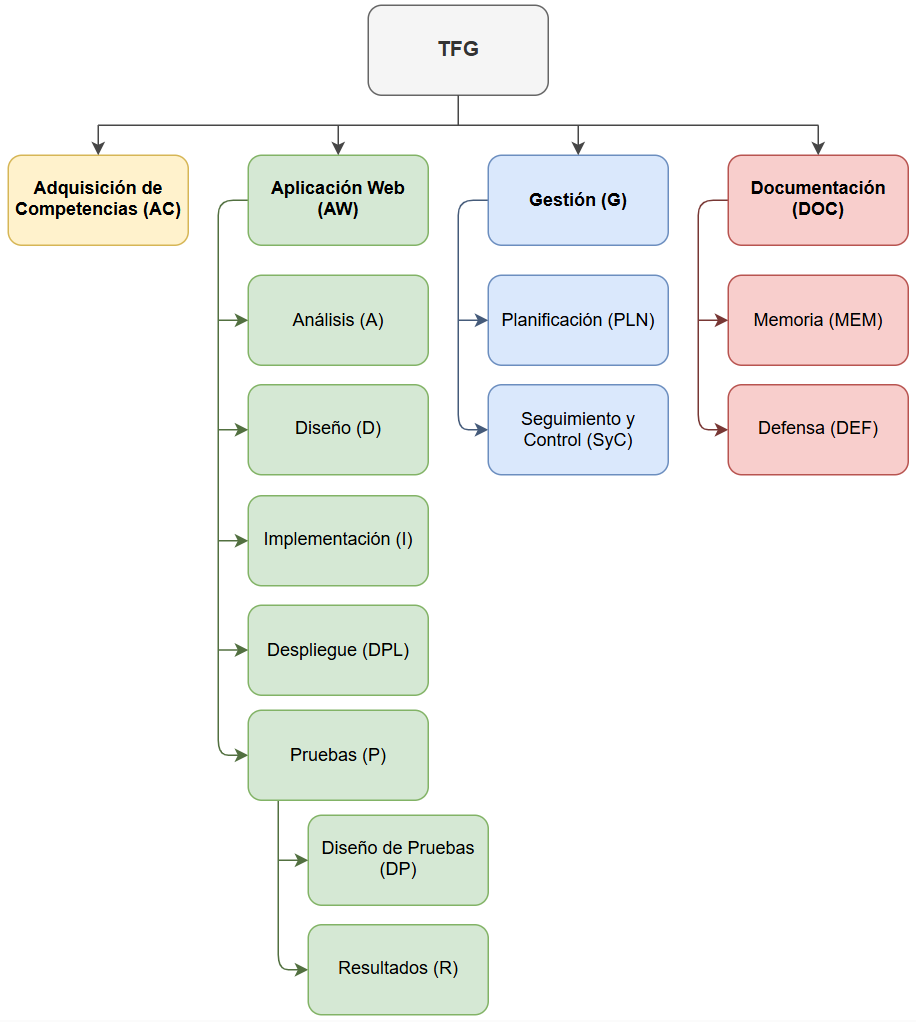
\includegraphics[width=0.65\textwidth]{figures/edt.png}
    \caption{Diagrama EDT con los paquetes de trabajo del proyecto.}
    \label{fig:edt}
\end{figure}

A continuación se detalla cada paquete de trabajo y las tareas correspondientes contenidas en cada una:

\subsubsection{Adquisición de Competencias (AC):}

Este paquete de trabajo incluye todas las tareas necesarias para adquirir el conocimiento sobre las tecnologías y herramientas para el desarrollo del proyecto.

\begin{itemize}[itemsep=0.2em]
    \item \textbf{AC.1:} Aprender \textit{TypeScript}, \textit{React.js} y \textit{Next.js} para el desarrollo de la aplicación web.
    \item \textbf{AC.2:} Estudiar el uso de \textit{Vercel} para el hosting y despliegue de la aplicación.
    \item \textbf{AC.3:} Hacer un reconocimiento inicial de la \textit{Web API} de \textit{Spotify}.
\end{itemize}

\subsubsection{Aplicación Web (AW):}

En este paquete se engloban todas las fases de desarrollo de la aplicación web, desde la planificación inicial hasta el despliegue final.

\begin{itemize}
    \item \textbf{Análisis (A):}
          \begin{itemize}
              \item \textbf{AW.A.1:} Estudiar y analizar en profundidad la \textit{Web API} de \textit{Spotify} para determinar el alcance y sus limitaciones.
              \item \textbf{AW.A.2:} Definir los requisitos funcionales y no funcionales del sistema.
              \item \textbf{AW.A.3:} Desarrollar los principales casos de uso del sistema.
          \end{itemize}

          \vspace{2em}

    \item \textbf{Diseño (D):}
          \begin{itemize}
              \item \textbf{AW.D.1:} Diseñar la arquitectura del sistema.
              \item \textbf{AW.D.2:} Crear un diagrama de componentes \textit{React} para establecer la jerarquía y realizar un diseño general de la interfaz de usuario.
              \item \textbf{AW.D.3:} Definir los diagramas de secuencia de los casos principales.
              \item \textbf{AW.D.4:} Realizar una gestión de la seguridad y asegurar que se implementarán las medidas definidas por \textit{Spotify} para el uso de la API.
          \end{itemize}

    \item \textbf{Implementación (I):}
          \begin{itemize}
              \item \textbf{AW.I.1:} Implementar el login de la página web, usando el protocolo \textit{OAuth 2.0} implementado por \textit{Spotify}.
              \item \textbf{AW.I.2:} Implementar el panel inicial (dashboard) de la web.
              \item \textbf{AW.I.3:} Implementar la sección principal de estadísticas.
              \item \textbf{AW.I.4:} Implementar la funcionalidad de cerrar sesión.
              \item \textbf{AW.I.5:} Realizar optimizaciones y correcciones en la implementación.
          \end{itemize}

    \item \textbf{Despliegue (DPL):}
          \begin{itemize}
              \item \textbf{AW.DPL.1:} Configurar el despliegue en \textit{Vercel} para crear un proceso automático de despliegue.
              \item \textbf{AW.DPL.2:} Monitorear el funcionamiento del despliegue y los logs.
          \end{itemize}

    \item \textbf{Pruebas (P):}
          \begin{itemize}
              \item \textbf{AW.P.DP:} Planificar y diseñar pruebas unitarias, de integración y de carga para evaluar el rendimiento y la estabilidad de la aplicación.
              \item \textbf{AW.P.R:} Realizar las pruebas planificadas y documentar los errores encontrados. En caso de que sea posible, implementar las correcciones necesarias.
          \end{itemize}
\end{itemize}

\subsubsection{Gestión (G):}

\begin{itemize}
    \item \textbf{Planificación (PLN):}
          \begin{itemize}
              \item \textbf{G.PLN.1:} Realizar una primera estimación de tiempos de las tareas generales.
              \item \textbf{G.PLN.2:} Establecer el alcance inicial del proyecto según las características del producto seleccionadas.
              \item \textbf{G.PLN.3:} Definir la planificación del proyecto.
              \item \textbf{G.PLN.4:} Revisar y, si fuera necesario, modificar la planificación.
          \end{itemize}
    \item \textbf{Seguimiento y Control (SyC):}
          \begin{itemize}
              \item \textbf{G.SyC.1:} Conversaciones y comentarios de la tutora a lo largo del desarrollo.
              \item \textbf{G.SyC.2:} Elaboración de un documento para registrar las actividades y dedicaciones realizadas a lo largo del proyecto.
              \item \textbf{G.SyC.3:} Comparación de los datos del seguimiento con los de la placificación, identificación de las desviaciones y riesgos significativos.
          \end{itemize}
\end{itemize}

\subsubsection{Documentación (DOC):}

Este paquete agrupa las tareas necesarias para la elaboración de la memoria y la preparación de la defensa del proyecto.

\begin{itemize}
    \item \textbf{Memoria (MEM):}
          \begin{itemize}
              \item \textbf{DOC.MEM.1:} Preparar el entorno de trabajo en \LaTeX\ utilizando \textit{Visual Studio Code} y establecer la estructura básica de la memoria a partir de la plantilla proporcionada por la facultad.
              \item \textbf{DOC.MEM.2:} Redactar la memoria.
          \end{itemize}
    \item \textbf{Defensa (DEF):}
          \begin{itemize}
              \item \textbf{DOC.DEF.1:} Identificar los puntos y conceptos clave que se presentarán en la defensa.
              \item \textbf{DOC.DEF.2:} Crear los elementos visuales de apoyo para la defensa.
              \item \textbf{DOC.DEF.3:} Preparar y ensayar la defensa.
          \end{itemize}
\end{itemize}

\cleardoublepage

\subsection{Dedicaciones}

A continuación, en la tabla \ref{tab:estimaciones_tareas}, se presentan las horas estimadas para las tareas descritas en el apartado anterior. También se muestran las sumas de las dedicaciones por paquete de trabajo y la suma total de horas que se espera que lleve el desarrollo del proyecto completo.

\begin{table}[H]
    \centering
    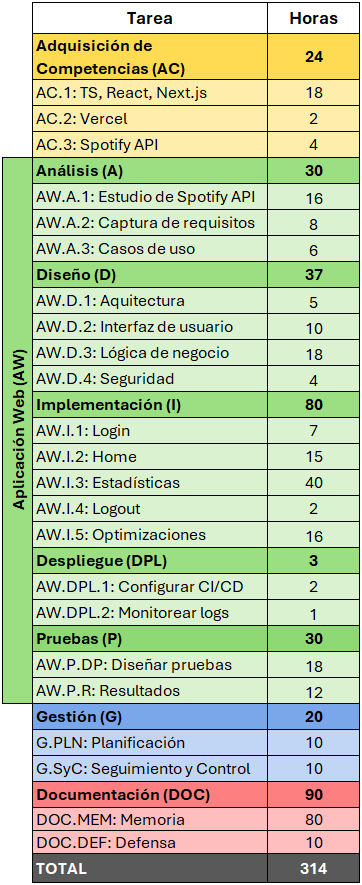
\includegraphics[width=0.55\textwidth]{figures/estimaciones_tareas.png}
    \caption{Tabla con las estimaciones de tiempo por paquete de trabajo y tarea del proyecto.}
    \label{tab:estimaciones_tareas}
\end{table}

\subsection{Dependencias entre Tareas}

En la figura \ref{fig:dependencias_tareas} se muestra un diagrama representando las dependencias que existen entre las diferentes tareas. De esta manera, se puede apreciar de forma visual las tareas que requieren la finalización de una o varias tareas para su comienzo.

\begin{figure}[H]
    \centering
    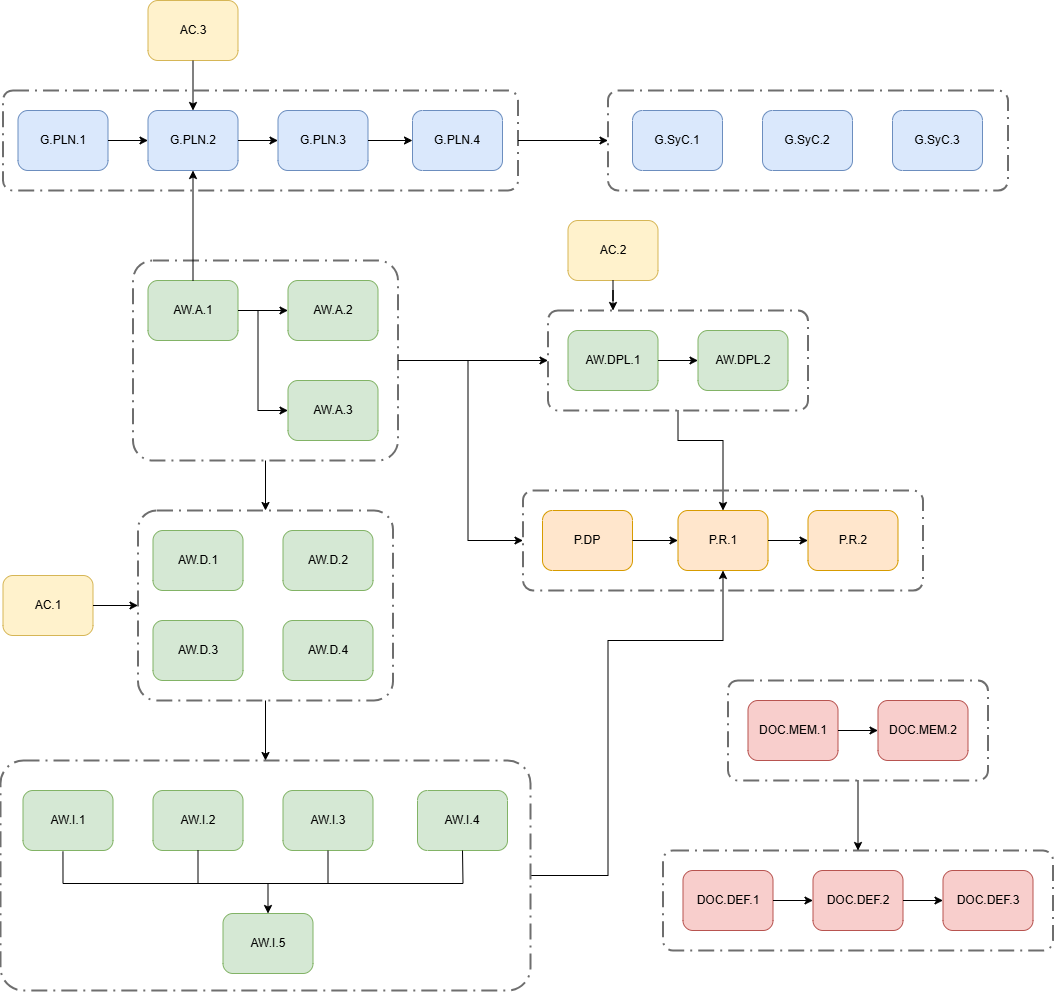
\includegraphics[width=\textwidth]{figures/dependencias_tareas.png}
    \caption{Diagrama de dependencias entre las tareas y paquetes de trabajo del proyecto.}
    \label{fig:dependencias_tareas}
\end{figure}

Como se puede apreciar, el proyecto debe iniciarse con las tareas de la planificación (paquete de trabajo \textbf{G.PLN}) y análisis (\textbf{AW.A}), al igual que el desarrollo de las tareas relacionadas con la memoria (\textbf{DOC.MEM}), que se realizan desde el inicio del proyecto hasta casi la finalización del TFG. Para ordenar temporalmente todas las tareas, en la siguiente sección se tratarán los periodos de desarrollo de cada una.

\newpage

\subsection{Periodos de Desarrollo e Hitos}

En esta sección se presenta el diagrama Gantt del proyecto (figura \ref{fig:gantt}), el cual ilustra los periodos de realización de las tareas y los paquetes de trabajo; siempre teniendo en cuenta las dedicaciones asignadas y las dependencias entre las tareas que se han establecido en la sección anterior. Además, se destacan los hitos del proyecto, permitiendo una visualización clara y organizada del cronograma planificado.

\begin{figure}[H]
    \centering
    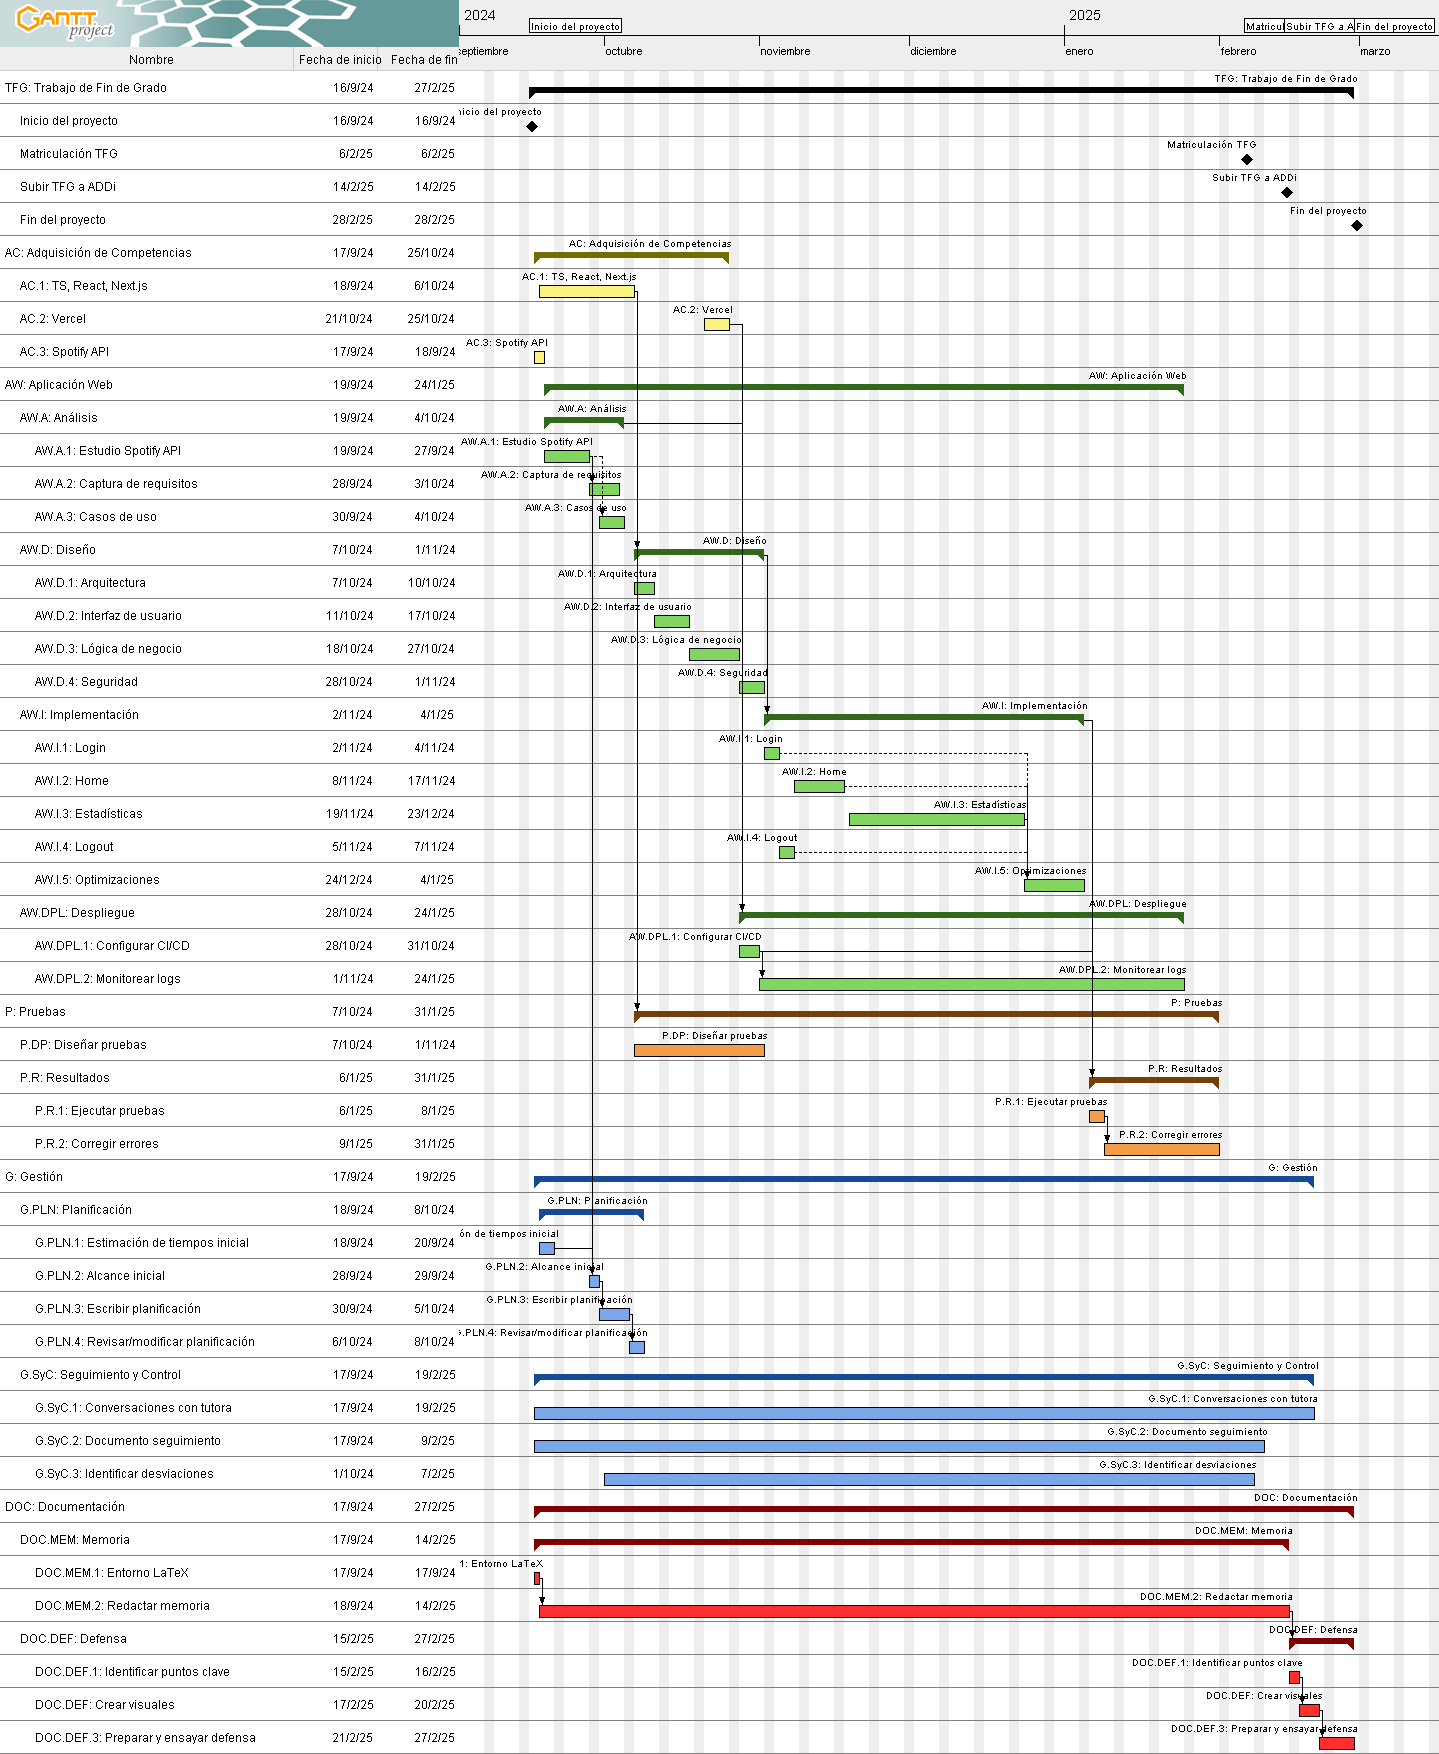
\includegraphics[width=\textwidth]{figures/gantt.png}
    \caption{Diagrama Gantt con los tiempos de realización de las tareas y paquetes de trabajo.}
    \label{fig:gantt}
\end{figure}

\section{Gestión de Riesgos}

La gestión de riesgos desempeña un papel crucial en cualquier proyecto, ya que permite anticiparse a posibles inconvenientes, definiendo estrategias adecuadas para minimizar su impacto sobre el proyecto.

A continuación, se presentan los riesgos identificados, especificando para cada uno de ellos la probabilidad de que se materialice, el impacto que podría ocasionar, las medidas implementadas para prevenirlos y las acciones que se llevarían a cabo en caso de que se acabe materializando alguno de ellos.

\subsection*{R01: Limitaciones con respecto a los datos disponibles de la API}
Este riesgo se refiere a la posible falta de datos suficientes o adecuados para implementar ciertas funcionalidades previstas, como estadísticas o visualizaciones concretas.

\begin{itemize}
    \item \textbf{Probabilidad}: Media.
    \item \textbf{Impacto}: Medio.
    \item \textbf{Prevención}: Analizar detenidamente los endpoints de la API antes de planificar funcionalidades dependientes de datos específicos.
    \item \textbf{Plan de mitigación}: Proponer gráficos o funcionalidades alternativas que no dependan de esos datos.
\end{itemize}

\subsection*{R02: Cambios en la política de acceso a la API}
Como \textit{Spotify} se reserva el derecho de modificar en cualquier momento las políticas de uso de su API, existe la posibilidad de que algunas funcionalidades del proyecto se vean afectadas o limitadas debido a cambios en los permisos o en la disponibilidad de ciertos endpoints.

\begin{itemize}
    \item \textbf{Probabilidad}: Baja.
    \item \textbf{Impacto}: Alto.
    \item \textbf{Prevención}: Revisar con frecuencia la documentación oficial y adaptar el proyecto a los permisos disponibles desde el inicio.
    \item \textbf{Plan de mitigación}: Ajustar el alcance del proyecto para trabajar con los datos que sigan siendo accesibles y documentar los cambios en la memoria del TFG.
\end{itemize}

\subsection*{R03: Interrupciones en la disponibilidad de servicios de terceros}
Este riesgo engloba posibles problemas de disponibilidad en servicios externos críticos para el proyecto, como la API de \textit{Spotify} o el servicio de hosting de \textit{Vercel}.

\begin{itemize}
    \item \textbf{Probabilidad}: Baja.
    \item \textbf{Impacto}: Alto.
    \item \textbf{Prevención}: Mantener una planificación que contemple margen suficiente para posibles retrasos causados por la indisponibilidad de estos servicios. Además, probar despliegues en un entorno local para avanzar en el desarrollo mientras el servicio de hosting se restablece.
    \item \textbf{Plan de mitigación}: Continuar con el desarrollo de los aspectos que no dependan de estos servicios y retomar las tareas una vez se solucione la interrupción.
\end{itemize}

\subsection*{R04: Incompatibilidad de versiones de las tecnologías a utilizar}
Este riesgo está relacionado con posibles problemas de compatibilidad entre \textit{TypeScript}, \textit{React}, \textit{Next.js} y las librerías utilizadas.

\begin{itemize}
    \item \textbf{Probabilidad}: Media.
    \item \textbf{Impacto}: Alto.
    \item \textbf{Prevención}: Investigar y verificar compatibilidades antes de seleccionar versiones específicas. Evitar usar, en la medida de lo posible, versiones muy recientes que puedan tener problemas de estabilidad y de soporte por parte de otras herramientas.
    \item \textbf{Plan de mitigación}: Actualizar o cambiar las herramientas o librerías problemáticas por alternativas compatibles y realizar pruebas exhaustivas después de cada cambio.
\end{itemize}

\subsection*{R05: Dificultad en el aprendizaje de las herramientas a utilizar}
Al trabajar con herramientas, frameworks y tecnologías con los que no se ha tenido un contacto previo, se pueden ocasionar retrasos por el proceso de aprendizaje.

\begin{itemize}
    \item \textbf{Probabilidad}: Media.
    \item \textbf{Impacto}: Medio.
    \item \textbf{Prevención}: Reservar un tiempo de adquisición de conocimientos y realizar pruebas antes de comenzar con las implementaciones críticas.
    \item \textbf{Plan de mitigación}: Consultar documentación oficial, foros o buscar ayuda en comunidades de desarrollo en línea para resolver dudas rápidamente. Si no es suficiente, se puede avanzar con otra tarea que no dependa de la resolución del problema actual, permitiendo ganar tiempo mientras se sigue investigando la solución al inconveniente técnico.
\end{itemize}

\subsection*{R06: Dificultad para compaginar el proyecto con las obligaciones académicas}
Este riesgo hace referencia a la posibilidad de tener problemas a la hora de gestionar el tiempo disponible para dedicar al proyecto, ya que se está cursando una asignatura en paralelo.

\newpage

\begin{itemize}
    \item \textbf{Probabilidad}: Media.
    \item \textbf{Impacto}: Alto.
    \item \textbf{Prevención}: Planificar un calendario detallado y realista que reserve horas específicas para trabajar en el proyecto, priorizando las tareas críticas.
    \item \textbf{Plan de mitigación}: Ajustar la planificación redistribuyendo tareas menos prioritarias y minimizando así el impacto en el desarrollo del proyecto.
\end{itemize}

% * He decidido no hacer la Gestión de Calidad
% \section{Gestión de Calidad}

\addtocontents{toc}{\protect\setcounter{tocdepth}{1}}

\section{Herramientas y Tecnologías}

Durante el desarrollo del TFG se usarán diferentes herramientas, tanto para la implementación de la aplicación web como en la planificación y redacción de la memoria. Cada una de ellas ha sido seleccionada por su idoneidad para la tarea en cuestión. A continuación se mencionan dichas herramientas y tecnologías, su función en el proyecto y una justificación de su selección.

\subsection{TypeScript}
Lenguaje de programación que extiende JavaScript, añadiendo un sistema de tipos estáticos y funcionalidades adicionales que mejoran la robustez y mantenibilidad del código. Permite detectar errores durante el desarrollo, en lugar de en tiempo de ejecución, lo que reduce significativamente los problemas en aplicaciones grandes y complejas.

En este proyecto, \textit{TypeScript} se utiliza como lenguaje principal para implementar la aplicación web, gracias a sus múltiples ventajas:
\begin{itemize}
    \item \textbf{Tipado estático}: Permite definir explícitamente los tipos de variables, funciones y componentes, evitando errores comunes como el mal uso de datos o la incompatibilidad entre módulos.
    \item \textbf{Mejor autocompletado y documentación}: Herramientas como \textit{VSCode} ofrecen un autocompletado más preciso y una navegación clara del código, mejorando la productividad del desarrollo.
    \item \textbf{Compatibilidad con JavaScript}: Al ser un superconjunto de JavaScript, es totalmente compatible con cualquier código JavaScript existente, facilitando la integración.
    \item \textbf{Detección temprana de errores}: Como ya se ha mencionado, gracias a su compilador, los errores se detectan antes de ejecutar el código, garantizando una mayor calidad en las entregas.
\end{itemize}

\subsection{React.js}
Biblioteca de JavaScript desarrollada por \textit{Facebook}, diseñada para la creación de interfaces de usuario modernas y dinámicas. Es ampliamente reconocida por su enfoque declarativo, que facilita la construcción de componentes reutilizables. En este proyecto, \textit{React.js} sirve como base para desarrollar la interfaz de usuario de la aplicación web, aprovechando su capacidad para gestionar de manera eficiente la interacción entre los componentes y el estado de la aplicación.

\subsection{Next.js}
Next.js es un framework de desarrollo web basado en \textit{React.js}, diseñado para facilitar la creación de aplicaciones modernas, escalables y de alto rendimiento. En este proyecto, se utiliza para implementar la página web principal, proporcionando funcionalidades avanzadas como el renderizado híbrido (estático y dinámico), rutas dinámicas y optimización automática de recursos.

El framework emplea varias tecnologías para garantizar un entorno de desarrollo eficiente y una construcción optimizada de la aplicación:
\begin{itemize}
    \item \textbf{SWC}: Compilador de alto rendimiento escrito en \textit{Rust} utilizado durante el proceso de construcción.
    \item \textbf{Turbopack}: Empaquetador moderno que reemplaza a \textit{Webpack}, ofreciendo tiempos de desarrollo significativamente más rápidos.
    \item \textbf{ESLint}: Herramienta integrada para el análisis estático de código, que garantiza la detección de errores y el cumplimiento de buenas prácticas.
    \item \textbf{Node.js}: Entorno de ejecución de JavaScript necesario tanto para el desarrollo como para la compilación y el despliegue de la aplicación.
\end{itemize}

\subsection{TailwindCSS}
Framework de CSS de utilidad que permite crear interfaces de usuario de manera rápida mediante clases predefinidas. Su integración con \textit{Next.js} permite una optimización automática de los estilos, eliminando clases no utilizadas durante el proceso de compilación para reducir el tamaño final del archivo CSS.

\subsection{Spotify Web API}
Siendo el principal servicio utilizado en este proyecto, es una interfaz de programación que permite acceder a diversos datos de usuario y a información relacionada con el contenido disponible en la plataforma de \textit{Spotify}. Esta API ofrece múltiples endpoints que proporcionan acceso a los datos, los cuales gozan de una muy buena documentación en la página web oficial.

\subsection{Git y GitHub}
\textit{Git} es un sistema de control de versiones ampliamente utilizado en el desarrollo de software, que permite gestionar y realizar un seguimiento de los cambios en el código fuente del proyecto de manera eficiente. Por su parte, \textit{GitHub} es una plataforma basada en la nube que facilita el almacenamiento y la colaboración en proyectos gestionados con \textit{Git}. Juntas, estas herramientas forman una combinación esencial en cualquier proceso de desarrollo de software, proporcionando un entorno robusto para el control de versiones y el respaldo seguro del código.

\subsection{Vercel}
Plataforma de hosting y despliegue continuo, optimizada para aplicaciones web basadas en frameworks como \textit{Next.js}, \textit{React.js}, \textit{Vue.js} y otros. En este proyecto, \textit{Vercel} se utiliza para alojar y mantener la página web, asegurando un proceso de despliegue automatizado gracias a su integración nativa con \textit{GitHub}.

Una de las principales ventajas de \textit{Vercel} es su integración directa con repositorios en \textit{GitHub}. Esto permite que cada vez que se realiza un cambio en el código fuente (como un \textit{push} en la rama principal), se active un flujo de trabajo automatizado para desplegar la versión más reciente de la aplicación. Aunque \textit{Vercel} cuenta con flujos de trabajo internos para automatizar los despliegues, también es posible personalizarlos utilizando \textit{GitHub Actions}, lo que ofrece un mayor control sobre el proceso de CI/CD.

Además de la facilidad de despliegue, \textit{Vercel} proporciona funcionalidades avanzadas que resultan beneficiosas para este proyecto:
\begin{itemize}
    \item \textbf{Renderizado optimizado}: Soporte nativo para el renderizado estático (\textit{Static Site Generation}) y dinámico (\textit{Server-Side Rendering}), fundamentales para proyectos basados en \textit{Next.js}.
    \item \textbf{Red global de distribución de contenido (CDN)}: Los recursos de la aplicación se sirven desde una red global de servidores, garantizando tiempos de carga rápidos para los usuarios en diferentes ubicaciones.
    \item \textbf{Escalabilidad automática}: La plataforma ajusta automáticamente los recursos según la demanda, lo que elimina la necesidad de gestionar manualmente la infraestructura.
\end{itemize}

\subsection{Visual Studio Code (VSCode)}
Editor de código empleado para el desarrollo del proyecto. Se trata de un editor de código abierto y gratuito, creado por Microsoft y diseñado para soportar una amplia variedad de lenguajes de programación y tecnologías. Para el beneficio del proyecto, cuenta con la integración nativa de \textit{TypeScript} y \textit{React.js}

Además, también se emplea para la edición en local de la memoria del TFG escrita en \LaTeX, siendo una mejor alternativa a otros editores específicos del lenguaje y la preferencia personal a los editores locales en comparación con las herramientas online como \textit{Overleaf}. La posibilidad de gestionar tanto el código de la aplicación como la memoria en un mismo entorno mejora significativamente la organización y productividad durante el desarrollo.

\subsection{\LaTeX\ (MikTeX)}
Sistema de preparación de documentos ampliamente utilizado en entornos académicos y técnicos por su capacidad para generar documentos de alta calidad tipográfica. En este proyecto, \LaTeX\ se utiliza para la escritura y edición de la memoria del TFG.

Para la compilación de los documentos, se emplea \textit{MikTeX}, una distribución de \LaTeX\ que incluye las herramientas necesarias para gestionar paquetes y generar archivos en formato PDF. Como ya se ha mencionado, esta distribución se combina con \textit{VSCode} para una agradable experiencia de edición.

\subsection{Chart.js, D3.js y Konva}
Librerías de visualización utilizadas en la sección de estadísticas de la aplicación web. \textit{Chart.js} permite crear gráficos interactivos de forma sencilla, como barras, líneas y áreas. \textit{D3.js} ofrece mayor control sobre la manipulación de datos y gráficos personalizados. Por último, \textit{Konva} se centra en la gestión avanzada de gráficos en \textit{canvas}, facilitando interacciones y animaciones en los elementos visuales.

\subsection{Jest.js y React Testing Library}
Herramientas utilizadas para realizar las pruebas de la aplicación. Jest.js es un framework de testing desarrollado por \textit{Facebook}, diseñado para realizar pruebas unitarias e integración en aplicaciones JavaScript y \textit{TypeScript}, permitiendo detectar y corregir errores antes del despliegue. Complementando a Jest, \textit{React Testing Library} es una biblioteca enfocada en pruebas de componentes de \textit{React}, priorizando la interacción del usuario sobre la implementación interna. Esta combinación permite validar tanto la lógica del código como el correcto comportamiento de los componentes en la interfaz.

\subsection{Microsoft Excel}
Herramienta muy popular para la edición de hojas de cálculo, ampliamente utilizada en diferentes ámbitos debido a su versatilidad y funcionalidades avanzadas. Gracias a su capacidad para generar tablas claras y visuales, se ha empleado para crear las tablas que se incluyen en la memoria del TFG, las cuales se exportan y adaptan fácilmente para su posterior integración en el documento de \LaTeX, complementando el contenido técnico con representaciones más visuales.

\subsection{Draw.io}
Herramienta web utilizada para la creación de diagramas incluidos en la memoria del TFG. Su interfaz intuitiva permite elaborar diagramas técnicos con facilidad. Estos diagramas ayudan a ilustrar conceptos del proyecto, facilitando la comprensión de los aspectos técnicos por parte del lector.

\addtocontents{toc}{\protect\setcounter{tocdepth}{2}}